%TODO: Zusammenfassen und Capacitor vs. Cordova etwas ausführen
% Implementierung vermutlich dann mit Capacitor, weil von Ionic so empfohlen


\section{Ionic / Cordova / Capacitor}
\label{sec:Frameworks_Ionic}

Das Ionic-Framework ist kein Cross-Plattform Framework, sondern ein UI-Toolkit.
Damit nterstützt Ionic die Cross-Plattform Entwicklung nur indirekt, indem insbesondere die Erstellung der Oberflächen vereinfacht wird.
Wie \autoref{fig:ionic_architecture} zeigt, ist Ionic auf ein unterlagertes Cross-Plattform Framework angewiesen, wenn Cross-Plattform Apps entwickelt werden sollen.
Hierfür unterstützt Ionic Apache Cordova und das vom Ionic-Team entwickelte Capacitor, wobei die Verwendung des moderneren Capacitor empfohlen wird.
Ionic lässt sich allerdings auch in reinen Webanwendungen nutzen \cite{Ionic_Docs}.
\begin{figure}[h]
    \centering
    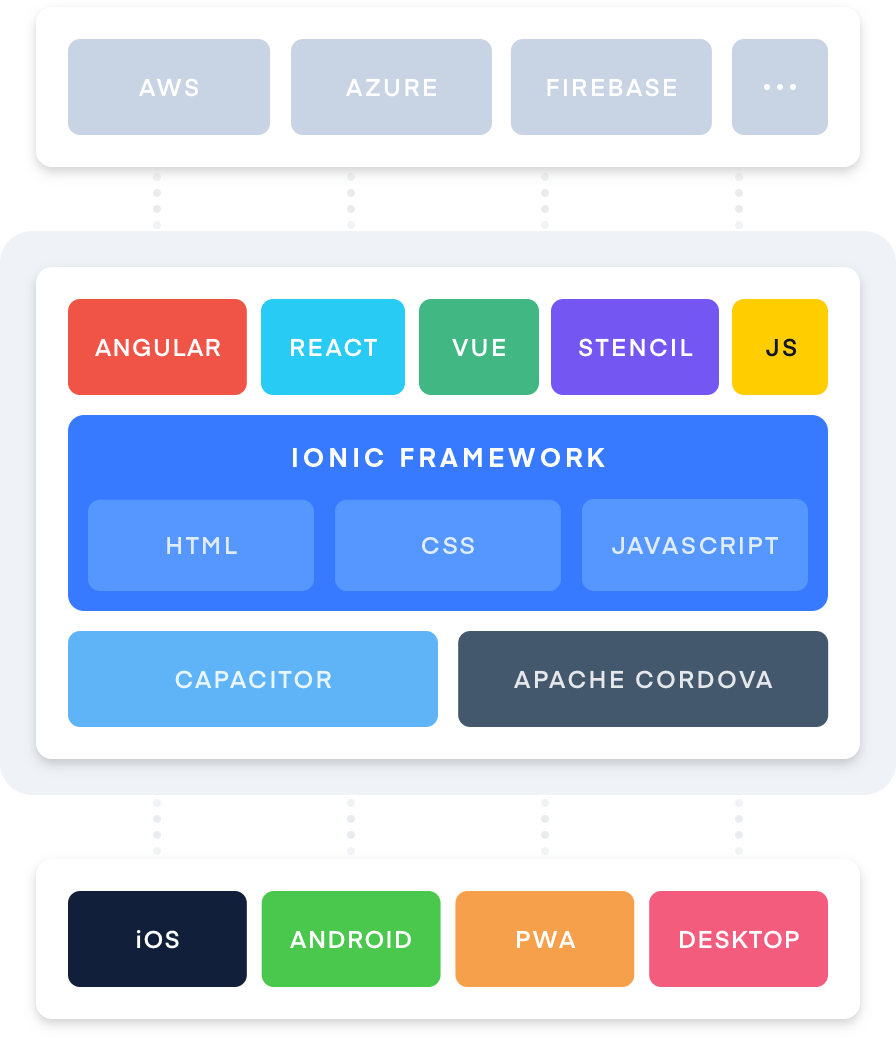
\includegraphics[width=0.72\textwidth]{ionic_architecture.png}
    \caption{Architektur des Ionic-Frameworks \cite{Ionic_Architektur}}
    \label{fig:ionic_architecture}
\end{figure}
Ionic stellt vor allem UI-Komponenten zur Verfügung, die plattformübergreifend genutzt werden können und automatisch dem Stil der jeweiligen Plattform angepasst werden.
Zur weiteren Vereinfachung bietet Ionic die Unterstützung der beliebten Frontend-Frameworks und Bibliotheken Angular, React und Vue.js.
Eine Ionic-Anwendung lässt sich auch mit anderen Frontend-Technologien oder komplett ohne Frontend-Framework erstellen \cite{Ionic_Docs, Ionic_EvaluationGuide}.
Zusätzlich erleichtert Ionic die Nutzung von TypeScript als Ersatz für JavaScript und bietet dafür typsichere Versionen von einigen Open-Source Plugins an. %TODO beleg
Ein weiterer Grund, der insbesondere Firmenkunden anspricht, sind die angebotenen Zusatzleistungen.
Für zahlende Kunden bietet Ionic persönliche Beratung und Support, ein eigenes \ac{CD} System und proprietäre Plugins für verschiedene Funktionen, die nicht über Open-Source Plugins abgedeckt werden können \cite{Ionic_EvaluationGuide}.


\subsection{Apache Cordova und Capacitor}
Die beiden unterstützen Cross-Plattform Frameworks Cordova und Capacitor sind sich im Allgemeinen sehr ähnlich.
Beide ermöglichen es, Webanwendungen in native Anwendungen einzubetten und über ein Plugin-System auf native \acp{API} zuzugreifen \cite{Ionic_Cordova_vs_Capacitor}.


Apache Cordova ist das deutlich ältere Framework und wird als Open-Source-Projekt von der Apache Software Foundation verwaltet.
Ursprünglich wurde Cordova von Nitobi, einer später von Adobe aufgekauften Firma, als kommerzielles Produkt entwickelt.
Eine Open-Source Version wurde 2011 an die Apache Software Foundation übergeben \cite{Steyer_Cordova}. %TODO quelle checken
Die kommerzielle Version des Frameworks wurde bis 2020 von Adobe als \textit{Adobe PhoneGap} vertrieben \cite{Adobe_PhoneGap_EOL}.
Aufgrund ihrer großen Ähnlichkeit wird in der Literatur meist nicht zwischen Adobe PhoneGap und der Open-Source Variante Apache Cordova unterschieden und beide Bezeichnungen werden teilweise synonym verwendet \cite{Steyer_Cordova,Manchanda_CrossPlatformFrameworks,Rieger_CrossPlatform_EvaluationFramework}. %TODO eventuell raus

Zur Unterstützung mehrerer Plattformen verwendet Cordova den Ansatz einer Hybrid Web App.
Jede Web-App, welche komplett mit \ac{HTML}, \ac{CSS} und JavaScript entwickelt wurde, lässt sich mit Cordova als native Anwendung verpacken.
\autoref{fig:cordova_architecture} zeigt die Architektur, die sich durch die Einbettung einer Web-App in einer nativen App ergibt.
\begin{figure}[h]
    \centering
    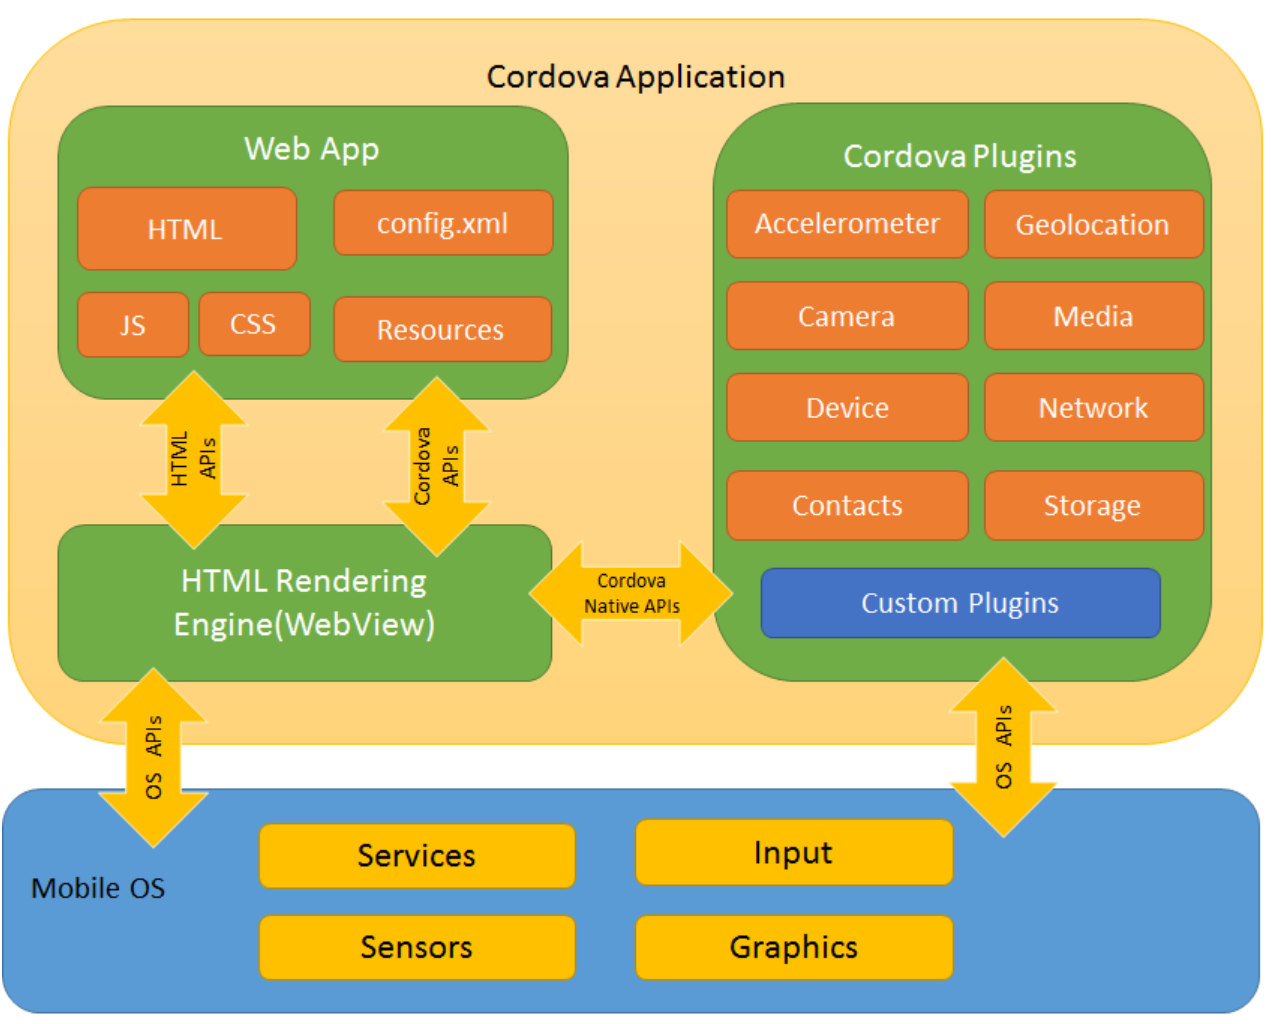
\includegraphics[width=0.85\textwidth]{cordova_architecture.png}
    \caption{Überblick über die Architektur einer Cordova-Anwendung \cite{Cordova_Overview}.}
    \label{fig:cordova_architecture}
\end{figure}



Theoretisch sind Web-Apps auch ohne den Einsatz von Cordova bereits plattformunabhängig, da sie auf verschiedenen Plattformen im Browser ausgeführt werden können.
Mit Cordova kann auf den Umweg über den Browser verzichtet werden und die Anwendung lässt sich über den App-Store der jeweiligen Plattform verbreiten.
Dazu verwendet Cordova eine Wrapper-Anwendung, welche die eigentliche Web-App in einer WebView ausführt.
Die WebView ist ein eingebetteter Webbrowser, der vom Betriebssystem bereitgestellt wird \cite{Steyer_Cordova}.
Zusätzlich können Cordova-basierte Anwendungen das bereits erwähnte und Plugin-System nutzen, um auf native Funktionen zuzugreifen \cite{Heitkoetter_CrossPlatform_Comparison}.
Der Zugriff auf native \acp{API} durch Plugins wird auch in \autoref{fig:cordova_architecture} verdeutlicht.
Für häufig verwendete Gerätefunktionen und \acp{API} stellt die Apache Software Foundation einige offizielle Plugins zur Verfügung.
Für eine Vielzahl von weiteren Funktionen sind Open-Source Plugins von anderen Anbietern verfügbar. 
Darüber hinaus erlaubt das Framework die Entwicklung eigener Plugins \cite{Cordova_Overview}.

Ein Plugin ist dabei eine JavaScript-Schnittstelle zu nativem, plattformspezifischem Code.
Aufrufe der Funktionen eines Plugins werden in der WebView zu Aufrufen der nativen Implementierung aufgelöst.
Der native Code muss die JavaScript-Schnittstelle implementieren, ist aber ansonsten in keiner Weise limitiert und kann alle verfügbaren \acp{API} verwenden.
Damit lassen sich alle Gerätefunktionen uneingeschränkt nutzen und bei Bedarf lässt sich die Performance von kritischer Funktionalität durch die Auslagerung in ein Plugin steigern.
Allerdings muss die Plugin-Funktionalität für jede zu unterstützende Zielplattform neu implementiert werden \cite{Steyer_Cordova}.
Werden ausschließlich Open-Source Plugins oder zugekaufte Plugins verwendet, kann der komplette Code der Anwendungen sowohl für Android als auch für iOS zum Einsatz kommen.
Allerdings sind einige Plugins nicht für alle Plattformen verfügbar oder funktionieren nicht auf allen Plattformen gleichermaßen \cite{Cordova_Plugin_Problem}.
Werden Funktionen benötigt, für die keine Plugins verfügbar sind, müssen eigene Plugins entwickelt werden.
Damit steigt der Entwicklungsaufwand enorm, was den Vorteil der Widerverwendung von Code schmälert.
Damit der große Vorteil der Cross-Plattform Entwicklung erhalten bleibt, sollten so wenige spezifische Plugins entwickelt werden müssen wie möglich \cite{Cordova_Development_Tips}.


Capacitor und Ionic werden vom gleichen Anbieter entwickelt und vertrieben.
Die Unterstützung von Capacitor ist in Ionic Projekten deshalb deutlich besser als die Unterstützung von Cordova \cite{Ionic_Cordova_vs_Capacitor}.
%TODO: capacitor Abschnitt



In \autoref{fig:ionic_architecture} ist gezeigt, dass Ionic sowohl auf Cordova als auch auf Capacitor aufsetzen kann.
Capacitor soll moderner sein als Cordova und verspricht eine bessere Unterstützung von \acp{PWA} und reinen Web-Apps.
Allerdings ist der Build-Prozess im Vergleich zu Cordova etwas aufwändiger, da die nativen Wrapper als separate Projekte verwaltet werden müssen \cite{Ionic_Cordova_vs_Capacitor}.
Grundsätzlich sind sich Cordova und Capacitor sehr ähnlich.
Durch die Kombination mit dem Ionic-Framework gibt es nahezu keine Unterschiede bei der App-Entwicklung, weshalb im Rahmen dieser Arbeit nicht auf weitere Unterschiede eingegangen werden soll.
\newline
\newline
Das Problem einer geringen Performance, das bereits in \autoref{sec:Frameorks_Cordova} erwähnt wurde, besteht vermutlich ebenfalls, da Ionic auf Cordova aufbaut.
In \cite{Biorn-Hansen_PerformanceOverhead_CrossPlatform} wird der Performance-Overhead von verschiedenen Cross-Plattform Frameworks bei typischen Aufgaben untersucht.
Hier wird deutlich, dass alle untersuchten Cross-Plattform Frameworks, darunter auch Ionic, wie erwartet eine schlechtere Performance aufweisen als eine native Anwendung.
Die untersuchten Szenarien beschränken sich auf Zugriffe auf Dateisystem, Kontaktlisten, Standort und Beschleunigungssensor.
Da die Anwendung, die im Rahmen dieser Arbeit entwickelt werden soll, keine dieser Funktionen benötigt und auch in anderen Quellen keine aussagekräftigen Tests der Netzwerk-Performance von Ionic-basierten Anwendungen vorhanden sind, können an dieser Stelle keine Aussagen über die zu erwartende Performance getroffen werden.




Das Cordova Framework ist schon lange verfügbar und unter Entwicklern etabliert.
Inzwischen hat sich deshalb eine große Community entwickelt.
Dadurch sind viele Ressourcen, wie spezielle Plugins, Anleitungen und ähnliches verfügbar, was die Entwicklung mit Cordova erleichtern kann.
Darüber hinaus sorgt der Einsatz von weit verbreiteten Web-Technologien wie zum Beispiel JavaScript für geringe Einstiegshürden \cite{Manchanda_CrossPlatformFrameworks,Singh_Cordova_vs_Native,Sasidaran_Survey_NativeHybrid}.
Durch die weite Verbreitung von JavaScript gibt es viele JavaScript-Bibliotheken und Tools, die in Verbindung mit dem Cordova Framework genutzt werden können.
%TODO: anpassen, vieles gilt auch für capacitor

%TODO: check
Die Beliebtheit des Frameworks ist allerdings laut der letzten Entwickler-Umfrage durch StackOverflow \cite{Stackoverflow_2022} vergleichsweise gering:
71,3 \% der Entwickler, die mit Cordova vertraut sind, geben an, das Framework nicht weiter einsetzen zu wollen.
Geringe Performance, vor allem durch die Interpretation von JavaScript-Code innerhalb der WebView und schlechte Unterstützung für Benutzerschnittstellen, die zur nativen \ac{UI} passen, sind Beispiele für häufig genannte Probleme bei Cordova \cite{Rieger_CrossPlatform_EvaluationFramework,Manchanda_CrossPlatformFrameworks,Heitkoetter_CrossPlatform_Comparison,Biorn-Hansen_PerformanceOverhead_CrossPlatform}.
Mit diesen Problemen kann vermutlich die geringe Beliebtheit erklärt werden.
